\section{Proposed Method}\label{sec:proposed_method}
In this section we introduce our proposed method. We first show our framework \modelname{} and then provide further details on the architectural composition.

%%%%%%%%%%%%%%%%%%%%%%%%%%%%%%%%%%%%%%%%%%%%%%%%%%%%%%%%%%%%%%%%%%
% Framework
%%%%%%%%%%%%%%%%%%%%%%%%%%%%%%%%%%%%%%%%%%%%%%%%%%%%%%%%%%%%%%%%%%
\subsection{Framework} \label{subsec:Framework}

\begin{figure}[t]
  \centering
  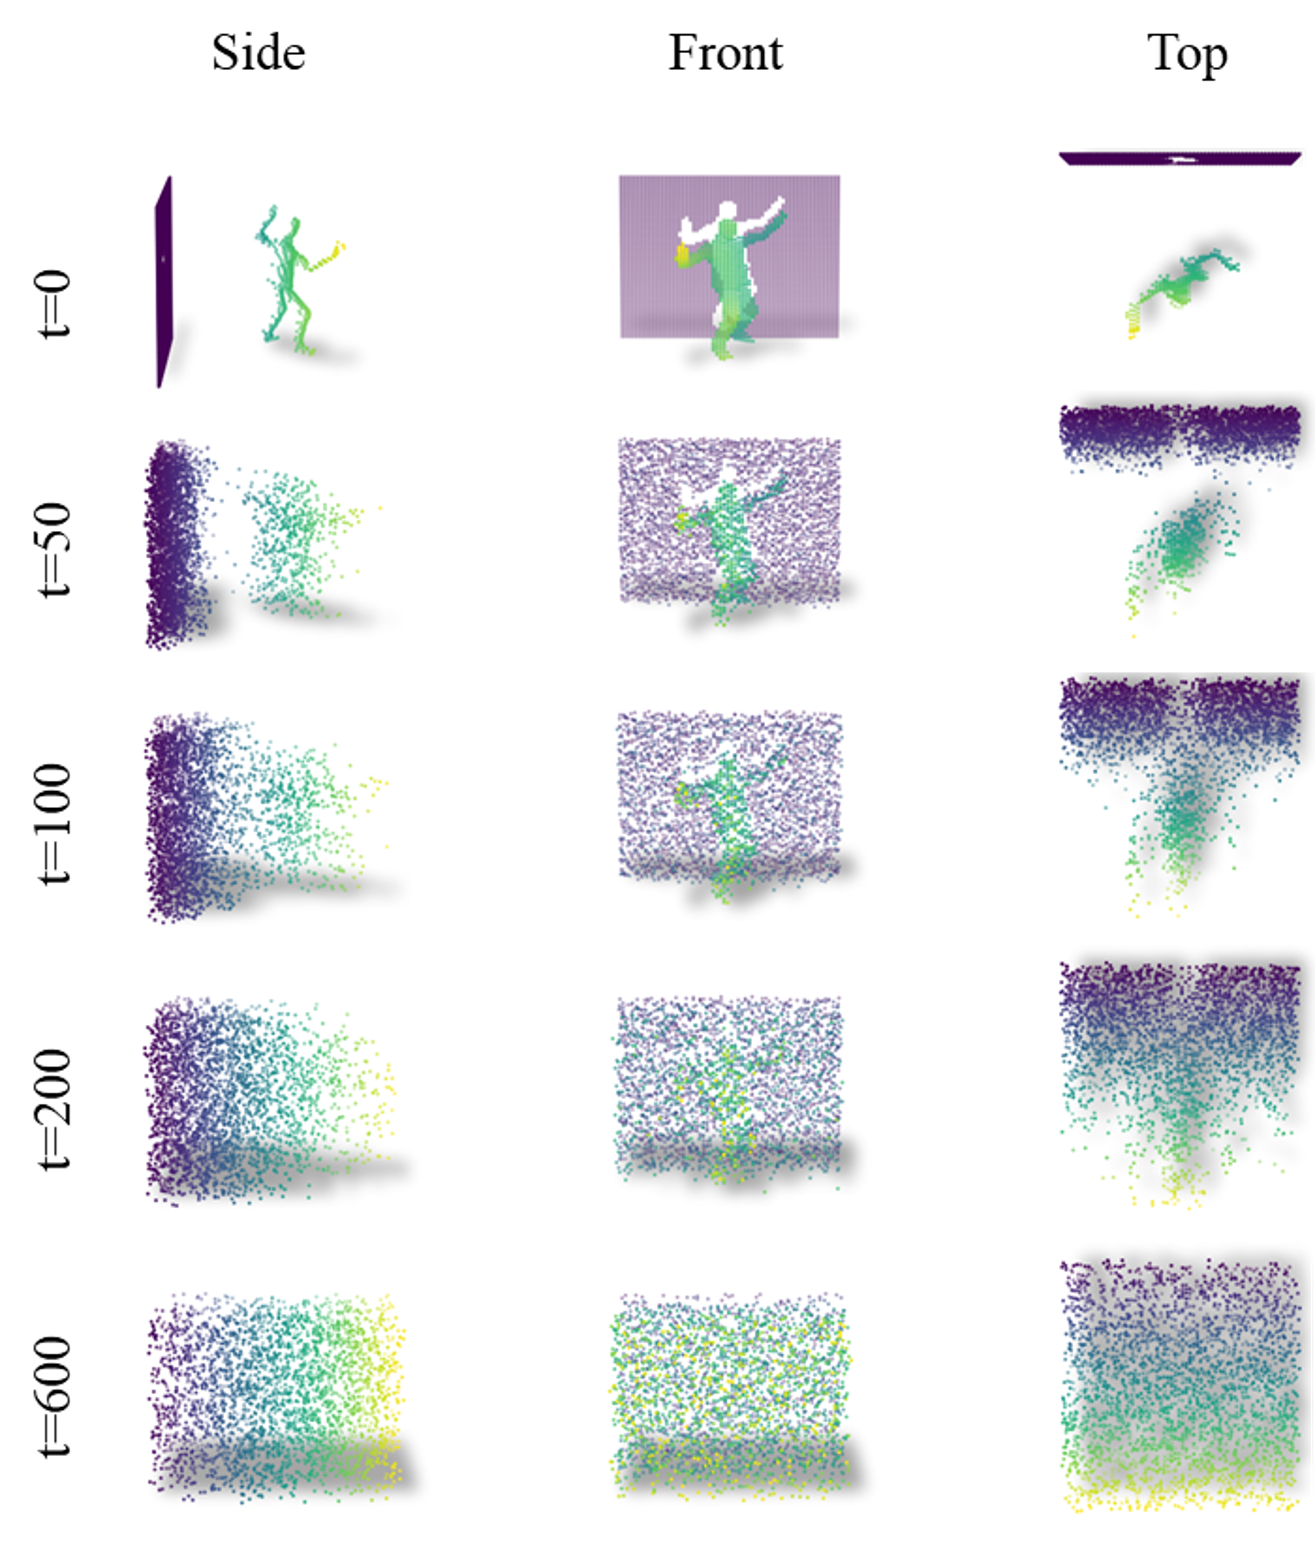
\includegraphics[width=0.99\linewidth]{illustrations/forward_diffusion.png}
  \caption{Forward diffusion process of a depth map represented as point cloud $P_{d}$ with a cosine beta schedule and with T=600 diffusion steps. Depth values are scaled to range from -1 to 1, with -1 being the background.}
  \label{fig:forward_diffusion}
\end{figure}

The \modelname{} framework is depicted in Fig. \ref{fig:framework}. We input an RGB image of a person with removed background (e.g. captured from a consumer camera device) and output an RGB-D image of that same person, with perspective projection. 

\begin{figure*}[t]
  \centering
  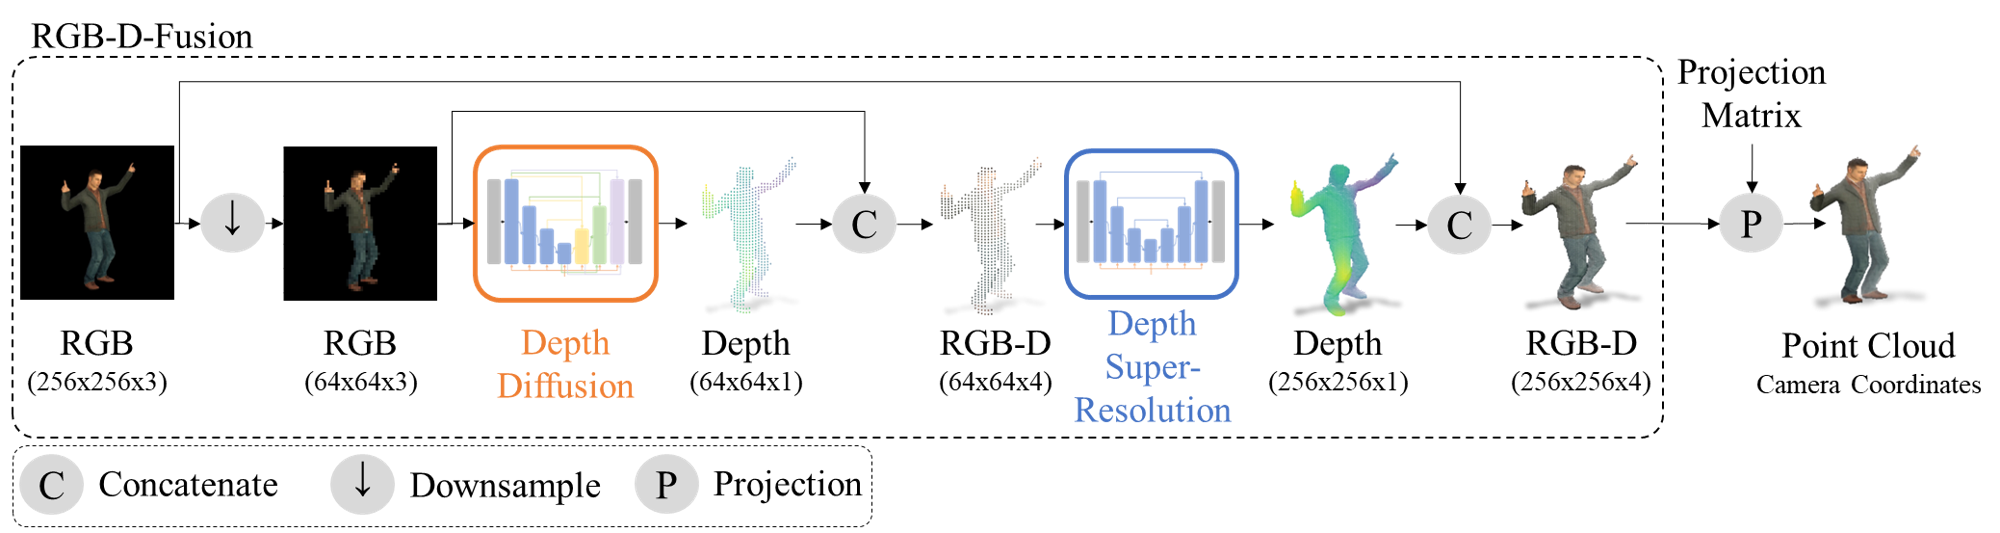
\includegraphics[width=0.99\textwidth]{illustrations/framework.png}
  \caption{\modelname{} framework. Our framework takes an RGB image as input and outputs an RGB-D image using perspective projection. We first downsample the input image from 256x256 to 64x64. We then predict the perspective depth map using a conditional denoising diffusion probabilistic model. We then combine the predicted depth map with the input RGB into an RGB-D image of resolution 64x64. We further apply a super-resolution model conditioned on the low-resolution RGB-D to obtain a high-resolution depth map. The predicted high-resolution depth map is combined with the input RGB to construct the final output: a high-resolution RGB-D image. To reconstruct the real depth in camera coordinates, a projection matrix can be applied if available.}
  \label{fig:framework}
\end{figure*}

Our framework consists of two stages: a depth prediction stage and a depth super-resolution stage. 
The first stage outputs a low-resolution perspective depth map for a given low-resolution RGB image. The second stage outputs a high-resolution depth map for a given low-resolution RGB-D input.

We first downsample the RGB input to a lower resolution of 64x64 pixels. We resample RGB data using bilinear resampling while for depth maps we apply nearest neighbors resampling to avoid undesired artefacts due to the large gradients introduced of the removed background. We feed the downsampled image into our first stage, a conditional diffusion model (details in section \ref{subsubsec:rgb_conditioned_depth_diffusion_model}) to predict the corresponding depth map. We combine the low-resolution RGB input with the predicted depth map to form an RGB-D image. The low-resolution RGB-D image is fed into our second stage, another conditional diffusion model (details in section \ref{subsubsec:rgbd_conditioned_depth_superresolution_diffusion_model}) to predict a high-resolution depth map. Finally, the predicted depth is combined with the initial RGB input to form the final RGB-D output.

Both our models, the depth diffusion model and the depth super-resolution model, perform the diffusion process on a depth map. The depth diffusion model samples a low-resolution depth map in 64x64 pixels, conditioned on a low-resolution RGB image. Our depth super-resolution model is conditioned on a low-resolution RGB-D image and samples a high-resolution depth map in 256x256 pixels. To obtain the depth in camera coordinates, one must further project the predicted output using a projection matrix if available.

We a apply a cosine beta schedule with $T=600$ for our depth diffusion model and $T=1000$ for our depth super-resolution model. Fig. \ref{fig:forward_diffusion} depicts the forward diffusion of a depth map represented as point cloud for various time steps and viewpoints.

In section \ref{sec:experiments} we perform various experiments to ablate and justify our architectural decision now introduced in further detail in section \ref{subsec:model_architecture}.

%%%%%%%%%%%%%%%%%%%%%%%%%%%%%%%%%%%%%%%%%%%%%%%%%%%%%%%%%%%%%%%%%%
% Model Architecture
%%%%%%%%%%%%%%%%%%%%%%%%%%%%%%%%%%%%%%%%%%%%%%%%%%%%%%%%%%%%%%%%%%
\subsection{Dataset}\label{subsec:dataset}

We created a custom dataset by rendering RGB-D images using perspective projection from high-quality 3D models of people \citep{volograms2021,escribano2022texture}. We randomly varied the camera's viewpoint, its field of view and its distance to the subject in such a way that the projected person covers 80\% of the image's height. Our dataset contains $\approx$ 25k samples. Each sample contains an RGB image of a person and its corresponding depth map. Both modalities have no background and have a spatial resolution of 256x256. 
The $\approx$ 25k samples are composed of 358 different subjects. We divide the dataset into a train set with 19,902 samples containing 315 subjects and a test set with 5,302 samples of 43 subjects. For better visualization of the depth maps, we illustrate them as point cloud $P_d = \{\left(u_{i}, v_{i},z_{i}\right) | i \in N \}$, where $N$ is the number of pixels of the depth map, $u_{i}$ and $v_{i}$ are the pixel coordinates and $d_{i}$ is the depth value. Likewise, an RGB-D image is represented as point cloud $P_{rgbd}= \{\left(u_{i}, v_{i}, d_{i},r_{i}, g_{i}, b_{i}\right) | i \in N \}$. In contrast, a colored point cloud in camera coordinates $P_{C}= \{\left(x_{i}, y_{i}, z_{i},r_{i}, g_{i}, b_{i}\right) | i \in N \}$ is defined by its 3D coordinates $x_i$, $y_i$ and $z_i$.

%%%%%%%%%%%%%%%%%%%%%%%%%%%%%%%%%%%%%%%%%%%%%%%%%%%%%%%%%%%%%%%%%%
% Model Architecture
%%%%%%%%%%%%%%%%%%%%%%%%%%%%%%%%%%%%%%%%%%%%%%%%%%%%%%%%%%%%%%%%%%
\subsection{Model Architecture} \label{subsec:model_architecture}
In this section we provide details on the two models that form our \modelname{} framework: the RGB conditioned depth diffusion model and the RGB-D conditioned depth super-resolution diffusion model.

%%%%%%%%%%%%%%%%%%%%%%%%%%%%%%%%%%%%%%%%%%%%%%%%%%%%%%%%%%%%%%%%%%
% Base Model
%%%%%%%%%%%%%%%%%%%%%%%%%%%%%%%%%%%%%%%%%%%%%%%%%%%%%%%%%%%%%%%%%%
\subsubsection{Base Model} \label{subsubsec:base_model}
Before we introduce the individual models we show the base model architecture from which we later derive our depth diffusion model and our depth super-resolution model.

In contrast to previous works \citep{dhariwal_diffusion_2021,nichol_improved_2021, ho_cascaded_2021} our base model architecture for the depth diffusion model is based on UNet3+ \citep{huang_unet_2020} and the architecture for our super-resolution model is based on the UNet architecture. A high level comparison is shown in Fig. \ref{fig:base_architecture}.

\begin{figure*}[t]
  \centering
  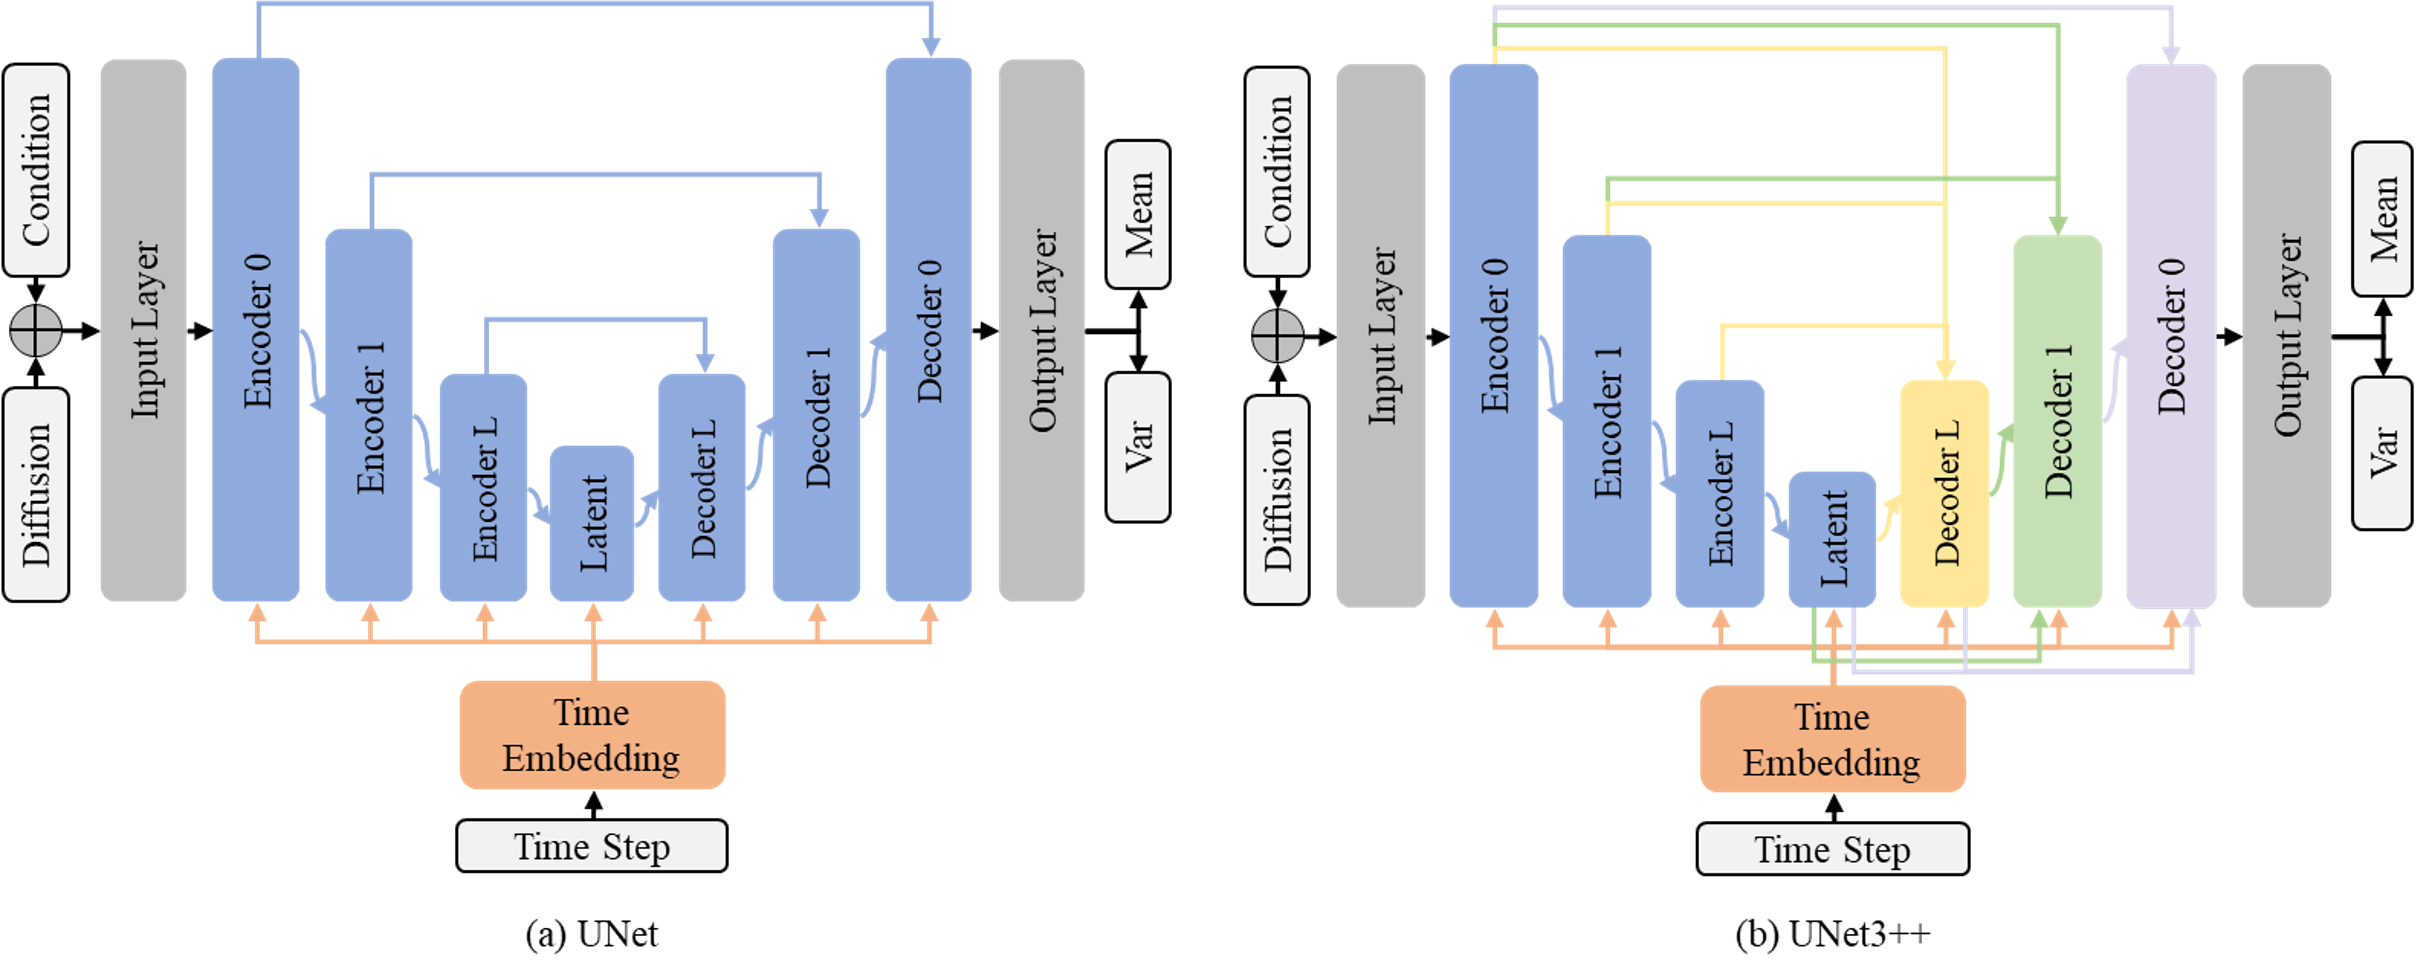
\includegraphics[width=0.99\textwidth]{illustrations/unet_combined.png}
  \caption{Comparison of our two base architectures. We condition our models on the time step $t$ of the diffusion process and on an additional condition input that is concatenated with the diffusion input. The diffusion input is the noisy sample. During training noise is gradually added to the diffusion input and gradually removed during sampling, while the condition is kept unchanged. Our models predict the mean and the variance of the conditioned diffusion input. The standard UNet architecture depicted in (a) simply connects the encoder and decoder stages with the same spatial resolution, while for the UNet3+ in (b), the decoder is connected to all encoder stages with the same or higher spatial resolution and all decoders with a smaller spatial resolution. Before concatenation, all feature maps are resampled to the same spatial resolution.}
  \label{fig:base_architecture}
\end{figure*}

Similar to \citep{dhariwal_diffusion_2021,nichol_improved_2021} we implement the stages of the model using multiple ResNet blocks followed by an optional multi-head attention block with 8 heads and a hidden dimension of 32 per head. For our latent space stage we implement standard attention by \cite{vaswani_attention_2017} and for stages with higher resolution we implement linear attention as proposed by \cite{wang_linformer_2020}. We also implement residual up and down-sampling blocks as suggested in BigGAN by \cite{brock_large_2019}.
We replace all normalization layers (i.e. batch normalization \cite{ioffe_batch_2015} and instance normalization \citep{ulyanov_instance_2017}) with group normalization \citep{wu_group_2018} with a groupsize of 8 and $\epsilon = 1e-05$ and only keep layer normalization \citep{ba_layer_2016} for all our attention blocks. 
As suggested by \cite{ioffe_batch_2015}, we remove all bias weights from our convolutional layers since the normalization layers introduce a learnable bias.
All activations are GeLU \citep{hendrycks_gaussian_2020} except for the softmax activations in the attention blocks.
We input the condition via concatenation with the noise input.
The time step information is input into each ResNet block (standard as well as in up and down sampling) using adaptive group normalization (AdaGN) \citep{dhariwal_diffusion_2021}.
Following \cite{liu_convnet_2022}, we increase the number of consecutive ResNet blocks in lower resolution stages and further apply stochastic depth \citep{huang_deep_2016} during training, to stochastically drop entire ResNet blocks to train an implicit ensemble of models.

%%%%%%%%%%%%%%%%%%%%%%%%%%%%%%%%%%%%%%%%%%%%%%%%%%%%%%%%%%%%%%%%%%
% RGB Conditioned Depth Diffusion Model
%%%%%%%%%%%%%%%%%%%%%%%%%%%%%%%%%%%%%%%%%%%%%%%%%%%%%%%%%%%%%%%%%%
\subsubsection{RGB Conditioned Depth Diffusion Model} \label{subsubsec:rgb_conditioned_depth_diffusion_model}
Our depth diffusion model is based on the UNet3+ architecture conditioned on a low-resolution (64x64x3) RGB image and generates a low-resolution depth map (64x64x1) when sampled from. 
The intention behind this architectural choice is to strengthen the decoder by using inputs from multiple resolutions of the UNet encoder, hence combining local and global features.
Corresponding experiments are performed in section \ref{subsec:experiements_depth_diffusion}.

%%%%%%%%%%%%%%%%%%%%%%%%%%%%%%%%%%%%%%%%%%%%%%%%%%%%%%%%%%%%%%%%%%
% RGB-D Conditioned Depth Super-Resolution Diffusion Model
%%%%%%%%%%%%%%%%%%%%%%%%%%%%%%%%%%%%%%%%%%%%%%%%%%%%%%%%%%%%%%%%%%
\subsubsection{RGB-D Conditioned Depth Super-Resolution Diffusion Model} \label{subsubsec:rgbd_conditioned_depth_superresolution_diffusion_model}

Our super-resolution diffusion model is conditioned on a low-resolution (64x64x4) RGB-D image and generates a high-resolution depth map (256x256x1) when sampled from. We use a UNet base architecture as depicted in Fig. \ref{fig:base_architecture}. The only difference is that before the low-resolution condition is fed into the model, we first upsample to the target resolution to match the resolution of the diffusion input. The RGB-D input is split into RGB and depth map, we then apply bilinear resampling for the RGB image and nearest neighbor resampling for the depth map and finally concatenate to a high-resolution RGB-D image (See Fig. \ref{fig:superres_model}). 
Corresponding experiments are performed in section \ref{subsec:experiements_superresolution}.

\begin{figure}[t]
  \centering
  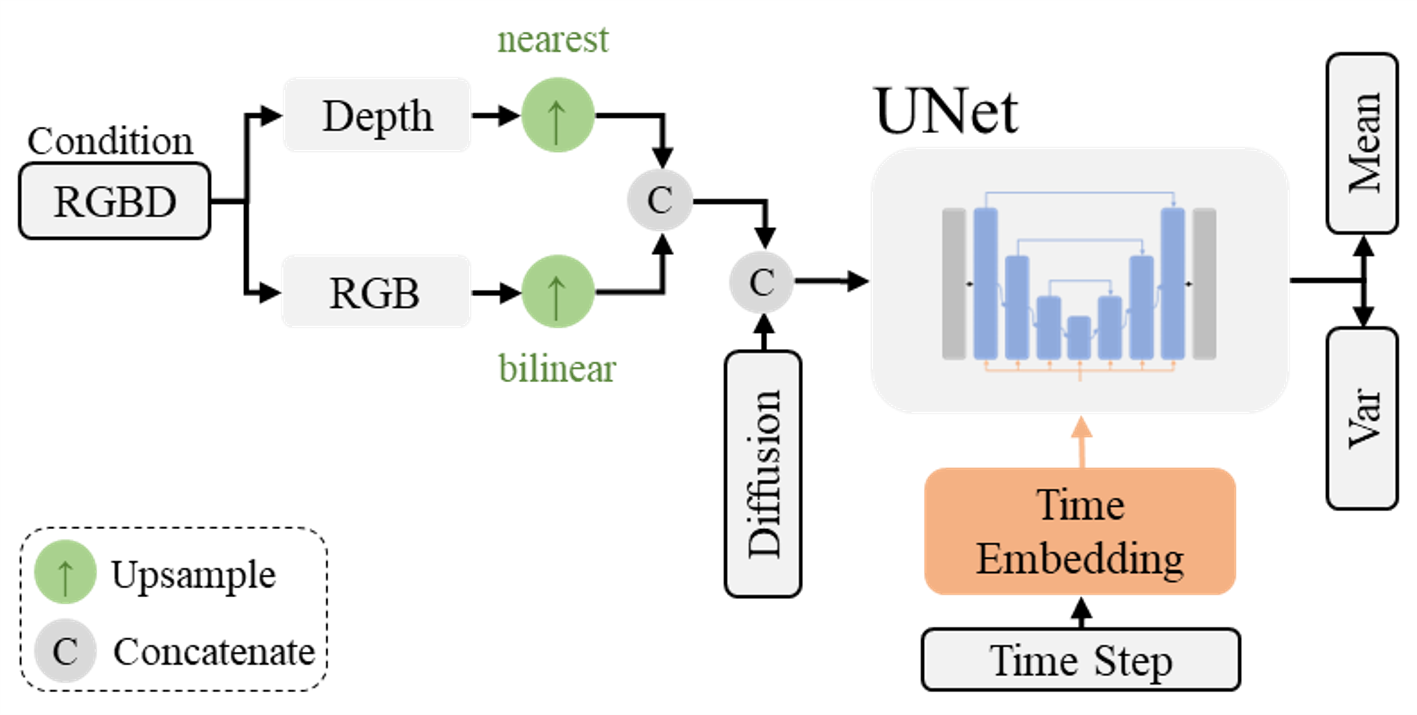
\includegraphics[width=0.99\linewidth]{illustrations/superres_model.png}
  \caption{Architecture of our depth super-resolution model. The low-resolution RGB-D image condition is split into its depth and RGB components, upsampled using nearest neighbor and bilinear resampling respectively, and combined again before it is fed into a UNet model.}
  \label{fig:superres_model}
\end{figure}

Compared to our depth diffusion model we make the following two assumptions: first, we assume that super-resolution is an easier task compared to depth estimation conditioned on a different modality, hence less parameters are required to learn this task. Second, high-resolution stages in the UNet architecture are more important than low-resolution stages since it is more important to focus on local features and not to have a global understanding of the image's content. 
Based on these assumptions and the fact that higher resolution images require more resources for training, we made the following design changes compared to our depth estimation network: first, we use a the UNet as a base architecture and increase the number of channels in the first stages of the UNet. This gives more importance on high-resolution stages and decreases the importance for low-resolution stages, while at the same time reducing the number of parameters. To extract more features for a given resolution, we increase the number of blocks within each stage. Second, we use the same number of stages in the UNet for our super-resolution from 64 to 128 as for 64 to 256, following the same argumentation of higher importance of high-resolution stages. The reduced number of stages, reduces the number of trainable parameters and computations required for the forward pass and lets us apply a higher batch size, hence speeds up the training and inference time.


%%%%%%%%%%%%%%%%%%%%%%%%%%%%%%%%%%%%%%%%%%%%%%%%%%%%%%%%%%%%%%%%%%
% Training Details
%%%%%%%%%%%%%%%%%%%%%%%%%%%%%%%%%%%%%%%%%%%%%%%%%%%%%%%%%%%%%%%%%%
\subsection{Data Augmentation} \label{subsec:data_augmentation}

During the training of our depth diffusion model we randomly scale and shift the RGB condition input.

For our depth super-resolution model we follow the suggestion of \cite{ho_cascaded_2021} and augment the RGB condition input with a Gaussian blur by convolving the image with a Gaussian 3x3 kernel with a standard deviation of $\sigma_{rgb} \sim \mathcal{U}_{[0,0.6]}$ with a probability of 0.5 in each epoch:
\begin{equation}
\label{eq:rgb_aug}
    rgb_{aug} = rgb * \epsilon_{rgb}
\end{equation}
where $\epsilon_{rgb} \sim \mathcal{N}\left(0,\sigma_{rgb}\right)$, $\epsilon_{rgb} \in \mathbb{R}^{3x3x3}$ and $rgb,rgb_{aug} \in \mathbb{R}^{HxWx3}$

In contrast to \cite{ho_cascaded_2021}, we further provide the depth as a condition input to our super-resolution model. Following the thoughts of \cite{ho_cascaded_2021} we augment the depth $d$ by adding Gaussian noise with an empirically determined standard deviation of $\sigma_{d} \sim \mathcal{U}_{[0,0.06]}$:
\begin{equation}
\label{eq:depth_aug}
    d_{aug} = d + \epsilon_{d}
\end{equation}
where $\epsilon_{d} \sim \mathcal{N}\left(0,\sigma_{d}\right)$ and $\epsilon_{d},d,d_{aug} \in \mathbb{R}^{HxWx1}$

Fig. \ref{fig:depth_gaussian_augmentation} shows the comparison of the depth without and with Gaussian additive noise, represented as a point cloud.

\begin{figure}[t]
  \centering
  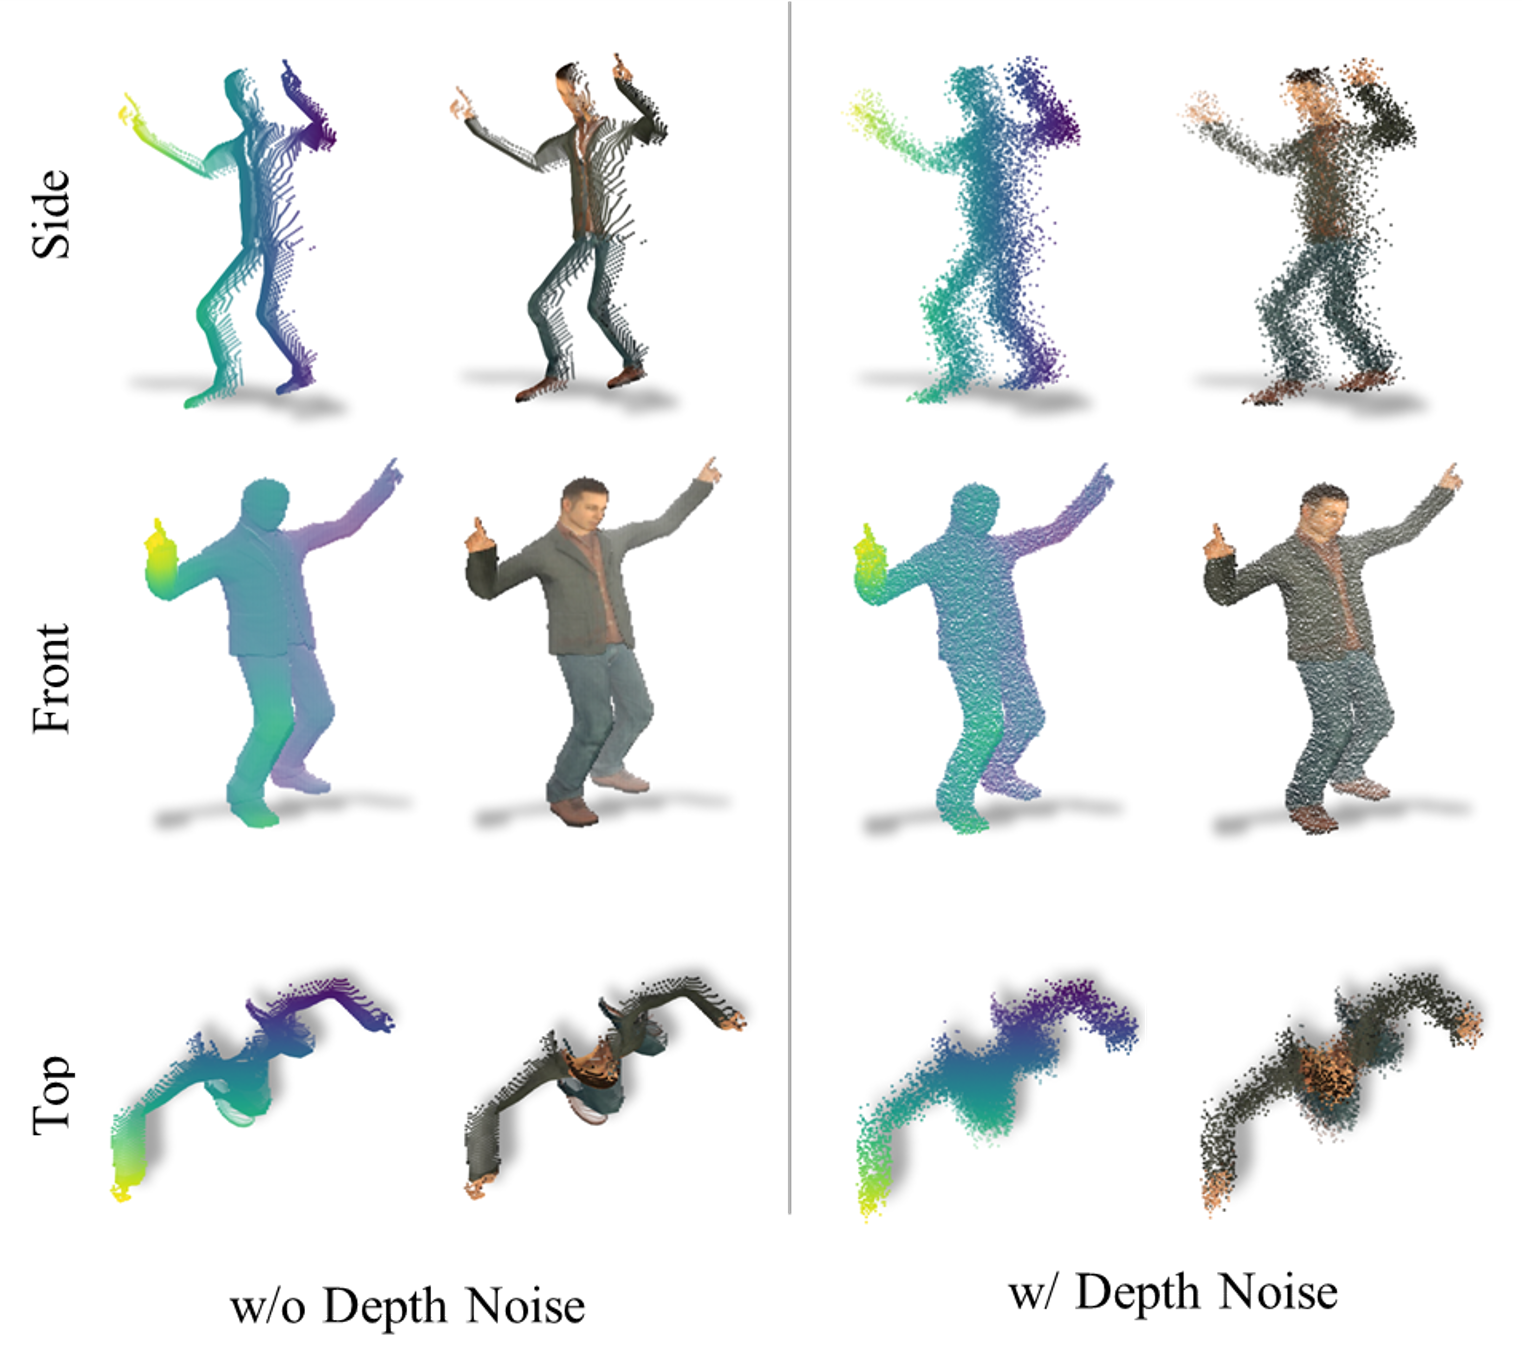
\includegraphics[width=0.99\linewidth]{illustrations/depth_noise.png}
  \caption{Comparison of a depth sample and an RGB-D sample without depth noise augmentation and with depth noise augmentation represented as point cloud $P_{d}$ and $P_{rgbd}$. We remove the points associated with the background for better representation.}
  \label{fig:depth_gaussian_augmentation}
\end{figure}
We further apply random scaling and shifting of the RGB-D condition input.